\begin{figure*}[!hbt]
  \centering
  \subfigure[Overall Runtime \textbf{(GPU)}]{
    \label{fig:temporal-compare--runtime-overall}
    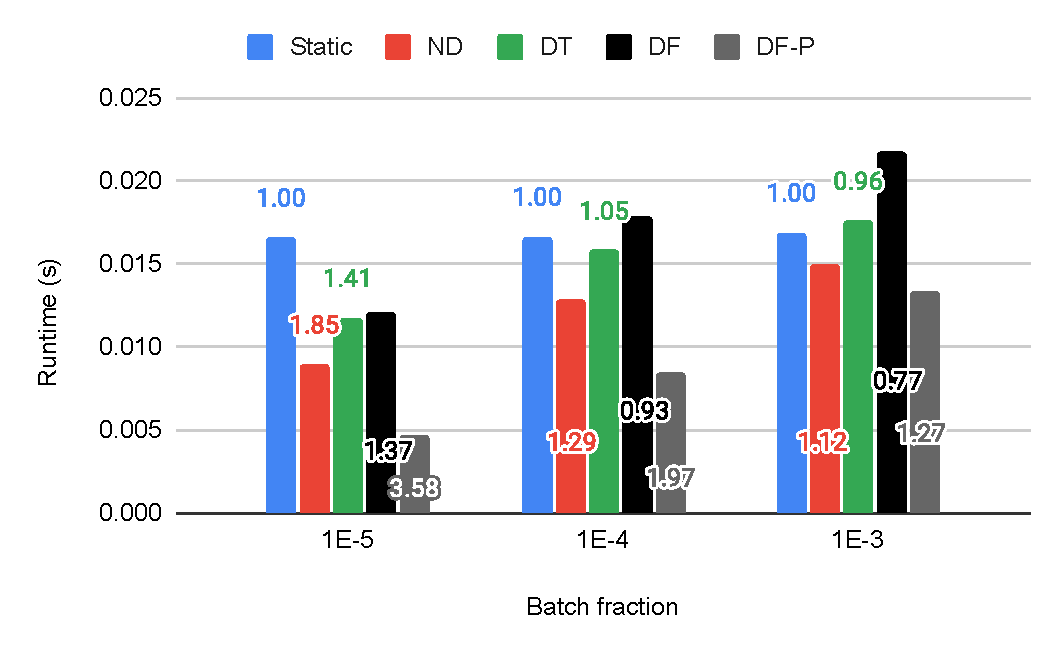
\includegraphics[width=0.48\linewidth]{out/temporal-summary-runtime-overall.pdf}
  }
  \subfigure[Overall Error in ranks obtained \textbf{(GPU)}]{
    \label{fig:temporal-compare--error-overall}
    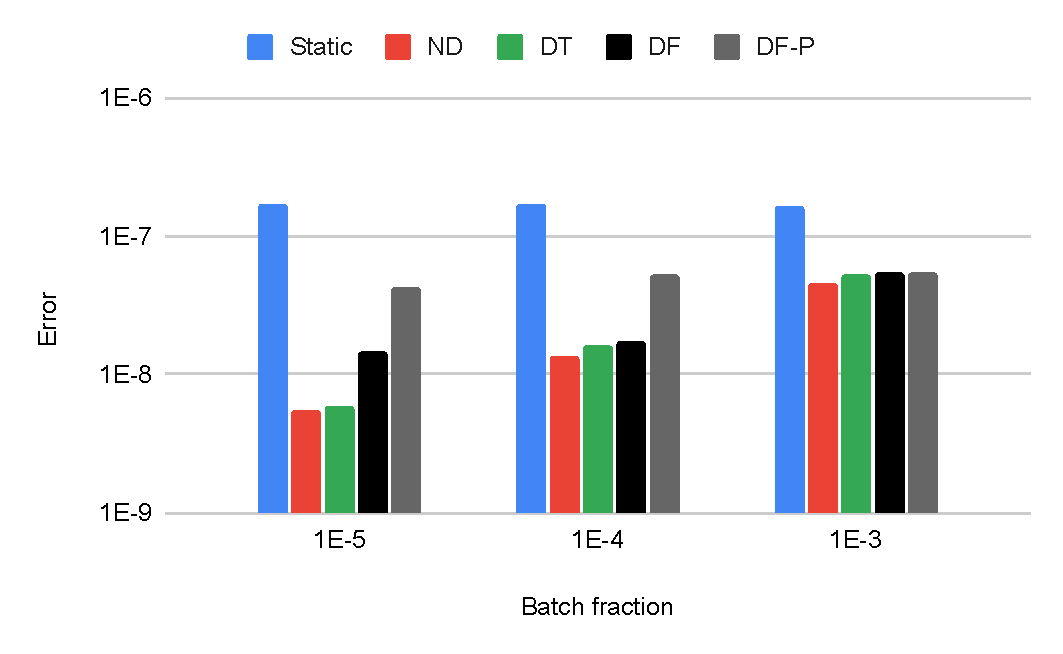
\includegraphics[width=0.48\linewidth]{out/temporal-summary-error-overall.pdf}
  }
  \subfigure[Overall Runtime \textbf{(CPU)}]{
    \label{fig:temporal-compare--runtime-overall-cpu}
    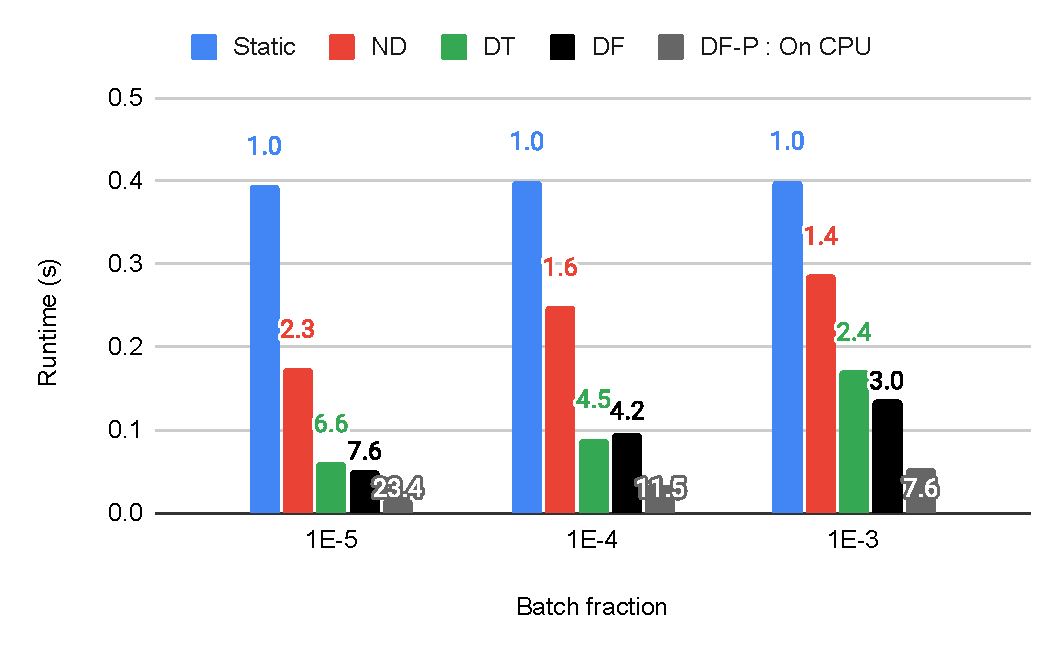
\includegraphics[width=0.48\linewidth]{out/temporal-summary-runtime-overall-cpu.pdf}
  }
  \subfigure[Overall Error in ranks obtained \textbf{(CPU)}]{
    \label{fig:temporal-compare--error-overall-cpu}
    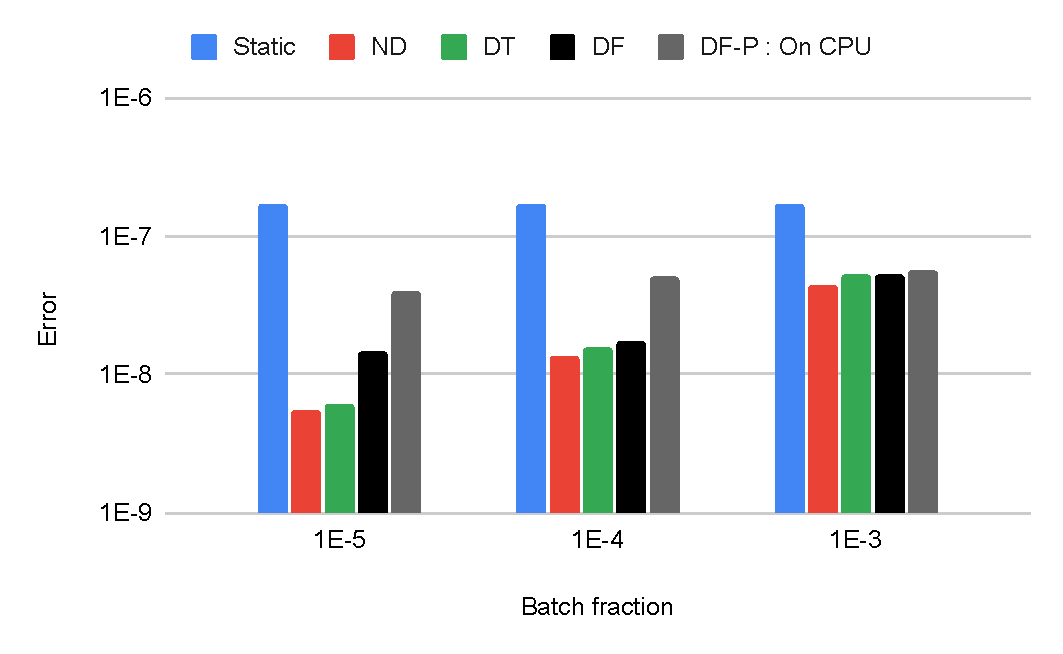
\includegraphics[width=0.48\linewidth]{out/temporal-summary-error-overall-cpu.pdf}
  } \\[-2ex]
  \caption{Mean Runtime and Error in ranks obtained with \textit{Static}, \textit{Naive-dynamic (ND)}, \textit{Dynamic Traversal (DT)}, our improved \textit{Dynamic Frontier (DF)}, and our improved \textit{Dynamic Frontier with Pruning (DF-P)} PageRank on real-world dynamic graphs, with batch updates of size $10^{-5}|E_T|$ to $10^{-3}|E_T|$. Here, (a) and (b) show the overall runtime and error across all temporal graphs, while (c) and (d) show the runtime and rank error for each approach (relative to reference Static PageRank, see Section \ref{sec:measurement}). In (a), the speedup of each approach with respect to Static PageRank is labeled. \su{TOWR}}
  \label{fig:temporal-compare}
\end{figure*}
